This section discusses the sources of the estimated gender differences. A major determinant is the choice of the alternative childcare arrangements. Estimated treatment effects are very similar across genders comparing treatment to staying at home full time. Males benefit much more from treatment relative to low-quality childcare compared to their benefits from treatment relative to staying at home. This result is consistent with previous research that shows (i) substantial gender differences resulting from attending low-quality childcare \citep{Kottelenberg-Lehrer_2014_Gender-Effects,Baker_Gruber_Milligan_2015_Noncog_Defects}; and (ii) that females are less sensitive to more stressful, low quality environments (see, e.g., \citealp{golding2016psychology,Autor-etal_2015_Family-Disadvantage}).

Table~\ref{tab:proportion-table-ranksign} shows the proportion of outcomes by category for which the male outcomes exceed those of females. In Appendix~\ref{appendix:propmales-females}, we present the analogous tables for staying at home and attending alternative preschool. We also partition the sample by father's presense, a potentially important moderator. Recall, we condition on baseline variables to control for selection into childcare for controls.\footnote{See Appendix~\ref{appendix:amethodology} \textbf{[JJH: Appendix E! On page 14 we say E!][We corrected and verified this Appendix reference.]} for a sensitivity study using other methods. They produce the same estimates, but are less precisely estimated.} Figure~\ref{fig:proportion-altpre} shows the proportions partitioned by alternative childcare setting. The males who stay at home do better than the females in cognitive and parenting measures, employment, and across all outcomes. Unlike the males who attend lower-quality alternative preschool, the males who stay at home have similar crime outcomes as the females. Given the important negative effects of male criminal activity, this finding highlights the magnitude of harm caused by low-quality alternative preschools for the males.

\begin{figure}[H]
\centering
\caption{Proportion of Outcomes Males $>$ Females, by Outcome Category, Partitioning by Alternative Childcare Setting}
\label{fig:proportion-altpre}
	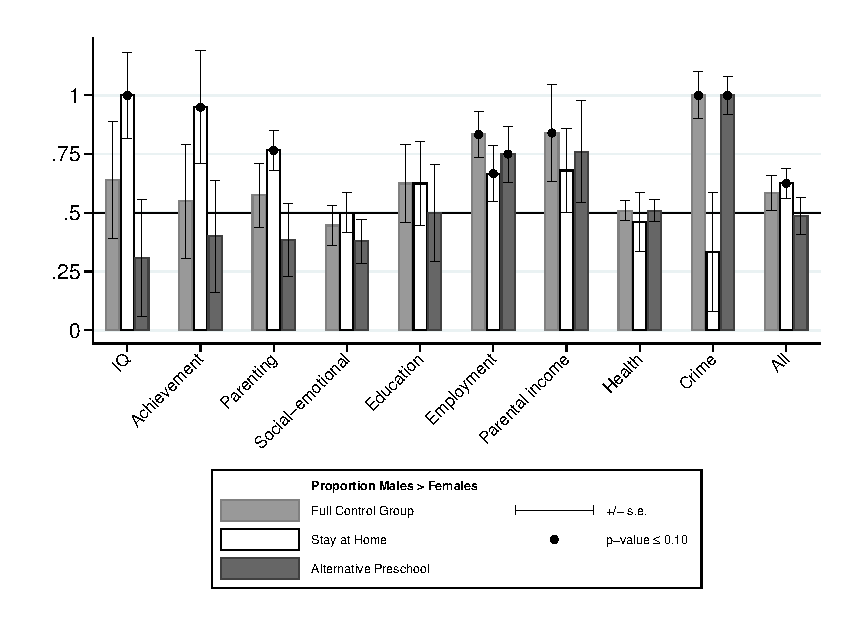
\includegraphics[width=\textwidth]{output/gendergaps-control-moderated-altpre}
\footnotesize \justify
Note: These plots show the proportion of outcomes, by outcome category, for which the males' mean is larger than the females' mean. The standard errors and the $p$-values are computed using 1,000 bootstraps. The $p$-values are one-sided and test the null hypothesis that the proportion of outcomes is greater than 50\% All outcome categories have higher values corresponding to socially desirable outcomes.
\end{figure}

In Appendix~\ref{appendix:genderdifferences}, we report estimates by whether or not the father is present (Figure~\ref{fig:proportion-fhome}). Parenting is better for control-group males when the father is absent. While this may seem contradictory, the parenting measure includes a scale that captures the absence of punishment. Those control-group males with an absent father tend to have higher parenting scores, especially for this scale, relative to those control-group males with a present father. In the treatment group, the males with a present father do better than those with an absent father. This hints at a complementarity between the father's parenting and the high-quality treatment. Besides this, few clear-cut patterns emerge. Father's presence interacted with treatment also favors males for IQ. Males in the control group do better when the father is absent in employment. \textbf{[JJH: The results for fathers present and absent are very difficult to interpret.][We added some explanation to help explain the parenting results. The fathers seem to be punishing the males more when they are in the control group, but not as much when they are in the treatment group. Also, please note that we changed the coding of some of the variables yesterday to make things more consistent (e.g. special education, retention, mental health outcomes reversed so that higher values mean socially positive results). We updated the text to reflect these changes.]}

\textbf{[JJH: Writing unclear. Is high good? Clarify.][A higher score is bad and it indicates having an external locus of control. A low score is good and corresponds to having an internal locus of control. It is the same scale. We clarified the description below.]}

Another measure of home environment is maternal locus of control which is measured when the subjects were 1.5 years old.\footnote{See \citet{Rotter_1966_PMGaA}. The researchers implementing ABC/CARE slightly modified the scale to be more appropriate for the population.} An internal locus of control, which is socially desirable, indicates feeling in control of future outcomes. In contrast, an external locus of control indicates feeling that outside forces determine future outcomes (e.g. luck). The test consists of pairs of opposing statements. The respondent chooses the statements that more closely align with her beliefs. One point is given for each statement the respondent selects that corresponds with an external locus of control. An example is: ``In the long run people get the respect they deserve in this world'' versus ``Unfortunately, an individual's worth often passes unrecognized no matter how hard he tries.'' If the respondent selects the second statement, she has a more external locus of control.  We define having an internal locus of control as scoring below the sample mean and having an external locus of control as scoring at or above the sample mean.

\textbf{[JJH: Internal + external = constant?][No, the locus of control is one scale. A low score corresponds to an internal locus of control, which is socially desirable. A high score corresponds to an external locus of control. We code it here such that anyone scoring below the mean has an internal locus of control, and anyone scoring above has an external one. We expanded the explanation to clarify.]} 

Figure~\ref{fig:proportion-mlocus} shows empirical results from conditioning on this variable. In the control group, an internal maternal locus of control promotes better outcomes for males across all outcome categories except health. Another way to state this is that males are more negatively affected if their mothers have an external locus of control than are females. This is consistent with the analyses of \citet{Schore_2017_IMHJ} and \citet{golding2016psychology}. Although locus of control does not necessarily measure depression, this finding corresponds with \citet{Beeghly-etal_2017_IMHJ}, who find that increased maternal depression lead to worse outcomes for young males relative to females.

\begin{figure}[!htbp]
\centering
\caption{Proportion of Outcomes Males $>$ Females, by Outcome Category, Dividing by Maternal Locus of Control}
\label{fig:proportion-mlocus}
\begin{subfigure}[h]{0.7\textwidth}
	\centering
	\caption{Control Group}
	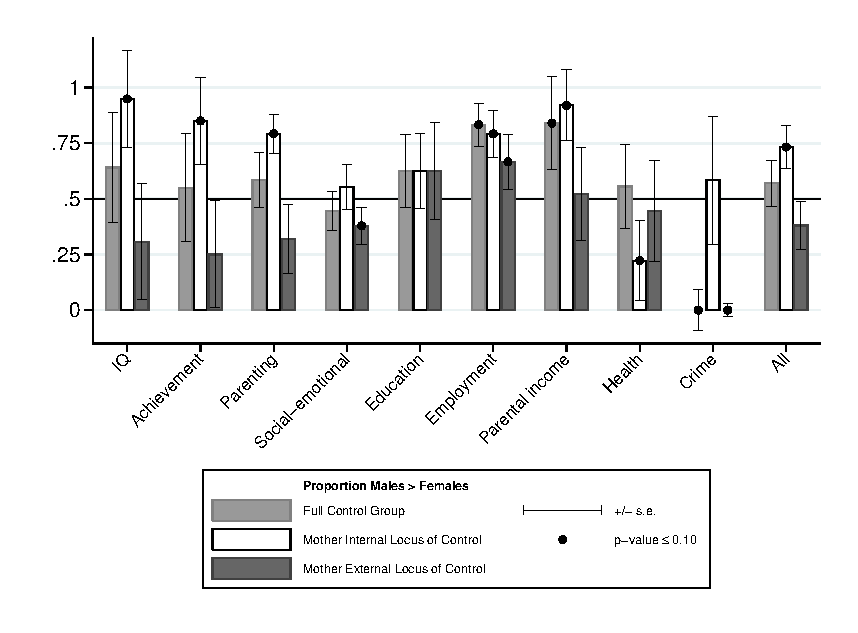
\includegraphics[width=\textwidth]{output/gendergaps-control-moderated-mlocus}
	\end{subfigure}
	
\begin{subfigure}[h]{0.7\textwidth}
	\centering
	\caption{Treatment Group}
	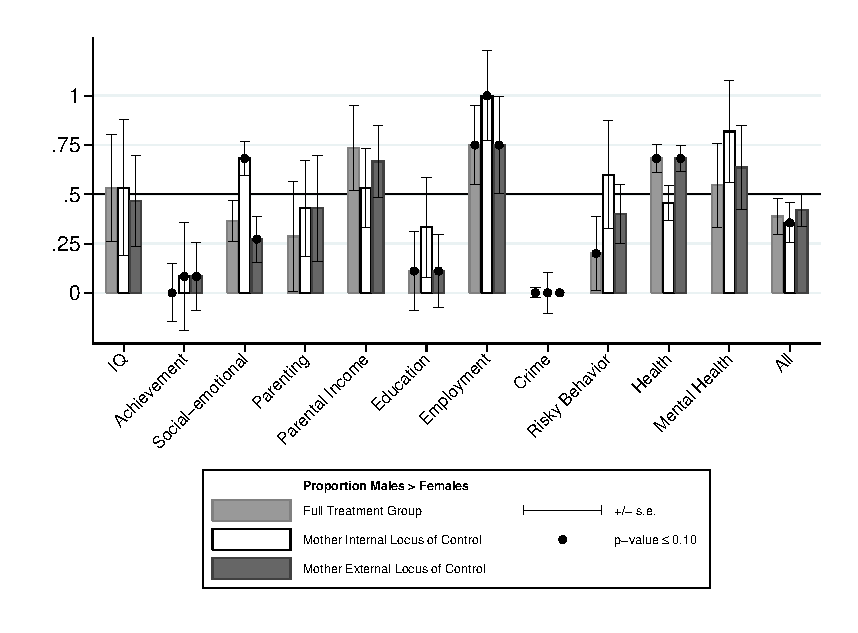
\includegraphics[width=\textwidth]{output/gendergaps-treatment-moderated-mlocus}
	\end{subfigure}
\footnotesize \justify
Note: These plots show the proportion of outcomes, by outcome category, for which the males' mean is larger than the females' mean. The standard errors and the $p$-values are computed using 1,000 bootstraps. The $p$-values are one-sided and test the null hypothesis that the proportion of outcomes is greater than 50\%. All outcome categories have higher values corresponding to socially desirable outcomes.
\end{figure}

Maternal locus of control moderates the treatment outcomes differently. Aggregating across outcomes, male outcomes are not much affected by the mother's locus of control if they attend ABC/CARE, while if they are in the control group, it does. This is especially stark for mental health outcomes. This suggests an important compensating role of enriched early childhood programs.



